%=====================================================================
%  CISC 7403 Cloud Computing - Project II
%  Scalable Web Service with Load Balancing
%
%  Compile:  latexmk -pdf main.tex      (or: pdflatex main.tex twice)
%
%  Every red \pending{...} marker and every placeholder image in figures/
%  must be replaced with the value / screenshot produced on the course
%  virtual machine (exact steps: ../../RUNBOOK_zh.md).
%=====================================================================
\documentclass[11pt,a4paper]{article}

\usepackage[T1]{fontenc}
\usepackage[utf8]{inputenc}
\usepackage{lmodern}
\usepackage[a4paper,top=1.8cm,bottom=1.8cm,left=1.9cm,right=1.9cm]{geometry}
\usepackage{graphicx}
\usepackage{booktabs}
\usepackage{caption}
\usepackage{subcaption}
\usepackage{xcolor}
\usepackage{listings}
\usepackage{enumitem}
\usepackage{tikz}
\usetikzlibrary{arrows.meta,positioning,fit,backgrounds,calc}
\usepackage[colorlinks=true,linkcolor=blue!50!black,urlcolor=blue!50!black,citecolor=blue!50!black]{hyperref}
\usepackage{float}

% Values that can only be produced by the on-VM experiment
\newcommand{\pending}[1]{\textcolor{red}{\textbf{[#1]}}}

\captionsetup{font=footnotesize,labelfont=bf,skip=2pt}
\setlength{\parskip}{0pt}
\setlength{\textfloatsep}{5pt plus 1pt minus 1pt}
\setlength{\intextsep}{5pt plus 1pt minus 1pt}
\setlength{\abovecaptionskip}{3pt}
\setlength{\emergencystretch}{2em}
\raggedbottom

\definecolor{codebg}{RGB}{247,247,249}
\lstdefinestyle{code}{
  backgroundcolor=\color{codebg},
  basicstyle=\ttfamily\scriptsize,
  commentstyle=\color{gray!80!black},
  keywordstyle=\color{blue!55!black},
  stringstyle=\color{teal!70!black},
  frame=single, rulecolor=\color{gray!35},
  breaklines=true, columns=fullflexible, keepspaces=true,
  upquote=true, showstringspaces=false,
  aboveskip=2pt, belowskip=2pt, xleftmargin=1pt, xrightmargin=1pt
}
\lstset{style=code}

\begin{document}
\small

%=====================================================================
% Cover page (excluded from the three-page limit)
%=====================================================================
\begin{titlepage}
  \centering
  \vspace*{3cm}
  {\Large\bfseries CISC 7403 --- Cloud Computing\par}
  \vspace{0.5cm}
  {\large Project II\par}
  \vspace{2cm}
  {\LARGE\bfseries Scalable Web Service with Load Balancing\par}
  \vspace{0.4cm}
  {\large Horizontal Scaling and Fault Tolerance\par}
  \vspace{2.2cm}
  \begin{tabular}{rl}
    \textbf{Team number:}    & \pending{XX} \\[3pt]
    \textbf{Team members:}   & \pending{Name 1 (student ID)} \\
                             & \pending{Name 2 (student ID)} \\[3pt]
    \textbf{Course section:} & CISC 7403 \\[3pt]
    \textbf{Date:}           & \pending{DD Month 2026} \\
  \end{tabular}
  \vfill
  {\footnotesize All measurements and screenshots in this report were produced on
   the course virtual machine using the code submitted together with it.}
\end{titlepage}

%=====================================================================
\section{System Architecture}
%=====================================================================
The system is three containers on one host: one Nginx container as the single
entry point and two identical backend containers built from the same application
image. Requests arrive at Nginx on host port 6120 and are forwarded in
round-robin order to \texttt{backend1} or \texttt{backend2}, which answer on the
internal port 8000. The replicas are stateless and interchangeable, so losing
one only reduces capacity and never breaks the service.

\begin{figure}[htbp]
\centering
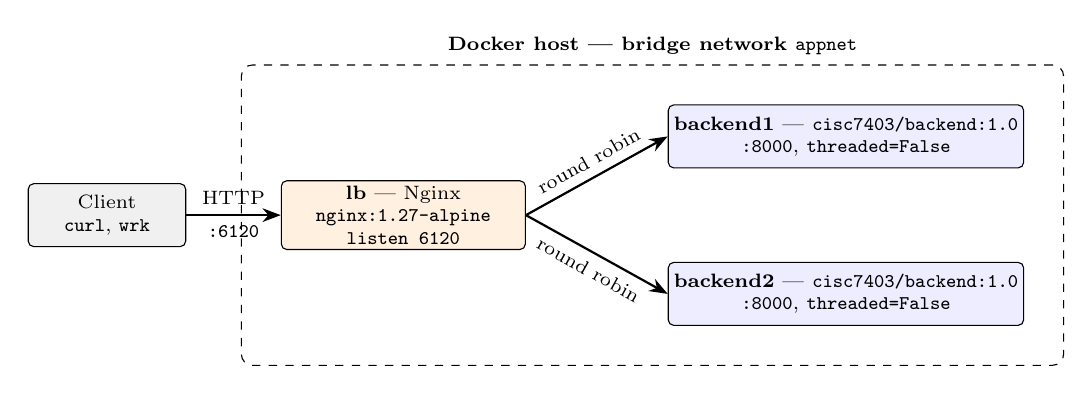
\begin{tikzpicture}[
    font=\scriptsize,
    box/.style={draw, rounded corners=2pt, align=center,
                minimum height=8mm, fill=white, inner sep=2pt},
    lb/.style={box, fill=orange!12},
    be/.style={box, fill=blue!7},
    host/.style={draw, dashed, rounded corners=4pt, inner sep=5mm},
    >={Stealth[]}
  ]
  \node[box, fill=gray!12, minimum width=20mm] (client) {Client\\\texttt{curl}, \texttt{wrk}};
  \node[lb, right=12mm of client, minimum width=31mm] (lb)
       {\textbf{lb} --- Nginx\\\texttt{nginx:1.27-alpine}\\\texttt{listen 6120}};
  \node[be, right=18mm of lb, yshift=10mm, minimum width=34mm] (b1)
       {\textbf{backend1} --- \texttt{cisc7403/backend:1.0}\\\texttt{:8000}, \texttt{threaded=False}};
  \node[be, right=18mm of lb, yshift=-10mm, minimum width=34mm] (b2)
       {\textbf{backend2} --- \texttt{cisc7403/backend:1.0}\\\texttt{:8000}, \texttt{threaded=False}};
  \draw[->, thick] (client) -- node[above]{HTTP} node[below]{\texttt{:6120}} (lb);
  \draw[->, thick] (lb.east) -- node[above, sloped, pos=0.5]{round robin} (b1.west);
  \draw[->, thick] (lb.east) -- node[below, sloped, pos=0.5]{round robin} (b2.west);
  \begin{scope}[on background layer]
    \node[host, fit=(lb)(b1)(b2),
          label={[font=\scriptsize\bfseries]above:Docker host --- bridge network \texttt{appnet}}] {};
  \end{scope}
\end{tikzpicture}
\caption{Architecture: one Nginx load balancer in front of two interchangeable
         backend replicas; only \texttt{lb} publishes a host port.}
\label{fig:arch}
\end{figure}

\begin{table}[htbp]
\centering
\footnotesize
\caption{Container inventory.}
\label{tab:containers}
\begin{tabular}{@{}llll@{}}
\toprule
Container & Image & Role & Host port \\
\midrule
\texttt{lb}       & \texttt{nginx:1.27-alpine}    & HTTP entry point, load balancing & \texttt{6120} \\
\texttt{backend1} & \texttt{cisc7403/backend:1.0} & Flask service instance \#1       & none \\
\texttt{backend2} & \texttt{cisc7403/backend:1.0} & Flask service instance \#2       & none \\
\bottomrule
\end{tabular}
\end{table}

%=====================================================================
\section{Implementation}
%=====================================================================
\paragraph{Backend service and image.}
\texttt{backend/app.py} is a Flask application on internal port 8000 with two
endpoints: \texttt{/} identifies the instance that served the request and
\texttt{/work} sleeps 50\,ms before answering. The instance name comes from
\texttt{INSTANCE\_NAME} (falling back to the container hostname), so both
replicas run exactly the same code. To guarantee that a container handles at
most one \texttt{/work} request at a time, the server runs with
\texttt{threaded=False}, one process and no reloader. Each request also writes
one line to stdout, which makes traffic visible in \texttt{docker compose logs}.
The image is built from \texttt{python:3.11-slim} and installs only Flask.

\begin{lstlisting}[language=Python,caption={Request handler and start-up (\texttt{backend/app.py}, abridged).},label={lst:app}]
@app.route("/work")
def work():
    time.sleep(WORK_DELAY_SECONDS)                     # 0.05 s
    _log("/work")
    return jsonify(instance=INSTANCE_NAME, hostname=HOSTNAME)

app.run(host="0.0.0.0", port=8000, threaded=False,      # one request at a time
        processes=1, use_reloader=False)
\end{lstlisting}

\paragraph{Nginx load balancer.}
The balancer is the official \texttt{nginx:1.27-alpine} image with
\texttt{nginx/nginx.conf} mounted read-only. Both backends are upstream servers
addressed by their Compose service names, which Docker's embedded DNS resolves
on the \texttt{appnet} network; the default round-robin policy spreads requests.
\texttt{proxy\_next\_upstream} makes Nginx retry the other server when the
chosen one refuses the connection, which keeps the service up during the
fault-injection test.

\begin{lstlisting}[caption={Load-balancer configuration (\texttt{nginx/nginx.conf}, abridged).},label={lst:nginx}]
upstream backend_pool {
    server backend1:8000;
    server backend2:8000;                    # service names, round robin default
}
server {
    listen 6120;
    location / {
        proxy_pass http://backend_pool;
        proxy_set_header Host            $host;
        proxy_set_header X-Forwarded-For $proxy_add_x_forwarded_for;
        proxy_connect_timeout 1s;
        proxy_next_upstream error timeout http_502 http_503 http_504;
    }
}
\end{lstlisting}

\paragraph{Compose deployment and networking.}
\texttt{docker-compose.yml} declares the three services and one user-defined
bridge network, \texttt{appnet}. Both backends share a YAML anchor, hence the
same build context and the same image tag; only \texttt{INSTANCE\_NAME} differs.
Only \texttt{lb} declares a \texttt{ports} mapping (\texttt{6120:6120}); the
backends declare \texttt{expose: 8000}, which is documentation and publishes
nothing to the host. The system starts with \texttt{docker compose up --build}.

% OPTIONAL deployment evidence: save the "docker compose ps" screenshot as
% figures/shot_deployment.png, then delete the two comment signs below.
% \begin{figure}[htbp]
% \centering
% \includegraphics[width=0.60\textwidth]{figures/shot_deployment.png}
% \caption{\texttt{docker compose ps}: three containers running, only \texttt{lb}
%          publishing port 6120.}
% \end{figure}

\begin{lstlisting}[caption={Excerpt of \texttt{docker-compose.yml}.},label={lst:compose}]
name: cisc7403-lb
x-backend: &backend                  # same context and image for both replicas
  image: cisc7403/backend:1.0
  build: {context: ./backend}
  networks: [appnet]
services:
  backend1:                  # backend2 is identical, only INSTANCE_NAME differs
    <<: *backend
    environment: {INSTANCE_NAME: backend1}
  lb:
    image: nginx:1.27-alpine
    ports: ["6120:6120"]
    volumes: ["./nginx/nginx.conf:/etc/nginx/nginx.conf:ro"]
    depends_on: [backend1, backend2]
networks:
  appnet: {driver: bridge}
\end{lstlisting}

%=====================================================================
\section{Load-Balancing Verification}
%=====================================================================
Ten requests were sent to the balancer after \texttt{docker compose up --build};
the \texttt{instance} field of each response was recorded with
\texttt{curl -s http://localhost:6120/}.

\begin{figure}[htbp]
\centering
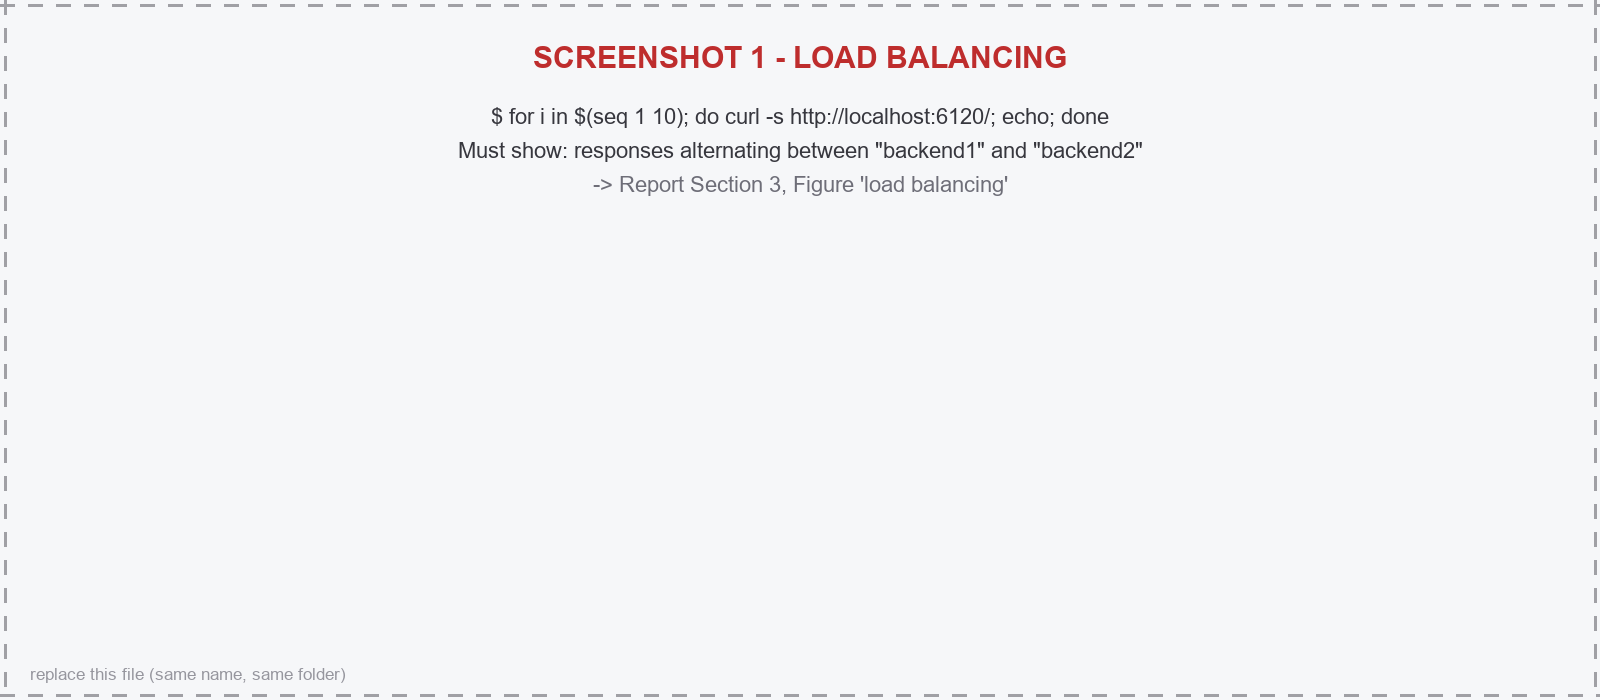
\includegraphics[width=0.60\textwidth]{figures/shot_load_balancing.png}
\caption{Ten consecutive requests through port 6120, answered alternately by
         \texttt{backend1} and \texttt{backend2}.}
\label{fig:lb}
\end{figure}

Of the \pending{N} requests, \pending{n1} were answered by \texttt{backend1} and
\pending{n2} by \texttt{backend2}. The split is close to even, so both replicas
are registered in the pool and Nginx really distributes the traffic instead of
always picking the first server. Strict alternation is not guaranteed with
reused connections, so only the overall balance is interpreted.

%=====================================================================
\section{Fault-Tolerance Experiment}
%=====================================================================
With both replicas serving traffic, \texttt{docker stop backend2} was executed
while the balancer kept running, the requests were repeated, and finally
\texttt{docker start backend2} brought the replica back.

\begin{figure}[htbp]
\centering
\begin{subfigure}[t]{0.48\textwidth}
  \centering
  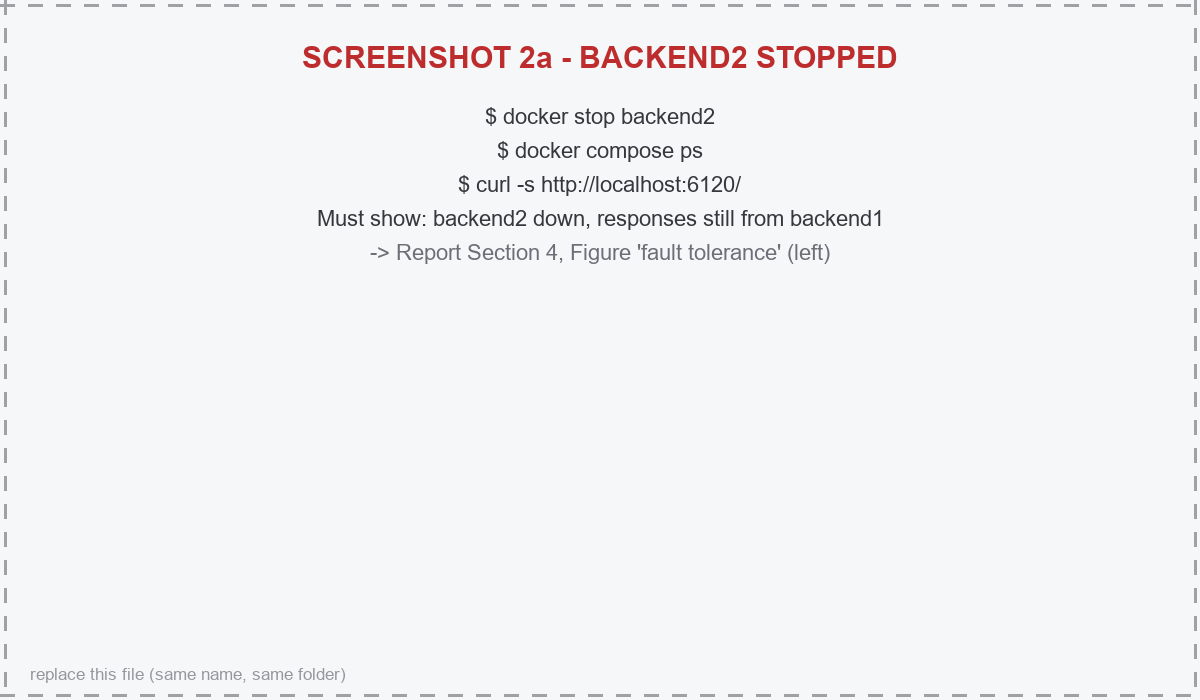
\includegraphics[width=\linewidth]{figures/shot_fault_stopped.png}
  \caption{\texttt{backend2} stopped.}
\end{subfigure}\hfill
\begin{subfigure}[t]{0.48\textwidth}
  \centering
  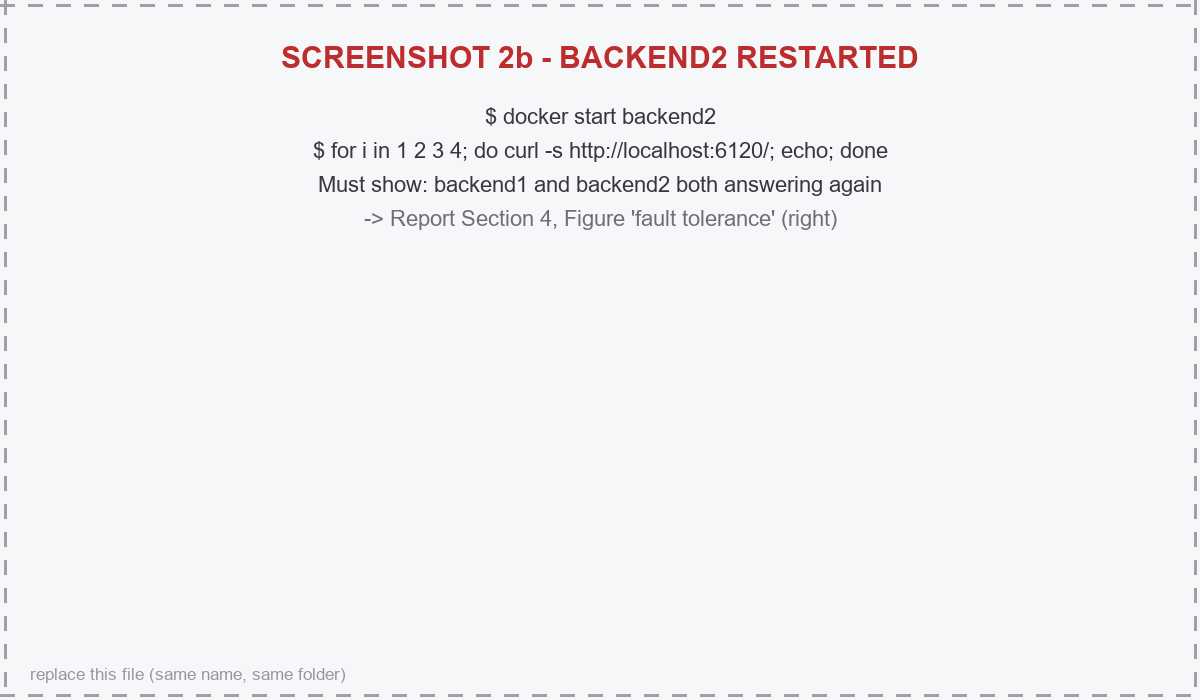
\includegraphics[width=\linewidth]{figures/shot_fault_restored.png}
  \caption{\texttt{backend2} restarted.}
\end{subfigure}
\caption{Fault tolerance: while one replica is down the service still answers
         through \texttt{backend1} (left), and after the restart both replicas
         receive traffic again (right).}
\label{fig:fault}
\end{figure}

All \pending{k} requests sent during the outage succeeded and were served by
\texttt{backend1}. The first request routed to the dead upstream failed at
connection level and was transparently retried on the healthy server, so the
client saw no error but may have observed a single slower response
(\pending{ms} average during the outage versus \pending{ms} in the healthy
state). After the restart the alternation returned without restarting Nginx,
because upstream names are resolved through Docker's DNS on every new
connection.

%=====================================================================
\section{Performance Experiment}
%=====================================================================
Both configurations were measured with the same workload through the balancer,
\texttt{wrk -t2 -c20 -d10s} against the URL \texttt{http://localhost:6120/work}.
The \emph{1 backend} case is the same application deployed from
\texttt{docker-compose.single.yml} with \texttt{nginx.single.conf}, i.e.\ the
second container \emph{and} the second upstream entry are removed, so no
request can be retried onto another instance.

\begin{table}[htbp]
\centering
\footnotesize
\caption{Throughput and average latency of \texttt{/work}
         (\texttt{wrk -t2 -c20 -d10s}, same VM for both runs).}
\label{tab:perf}
\begin{tabular}{@{}lcc@{}}
\toprule
Configuration & Throughput (req/s) & Average Latency (ms) \\
\midrule
1 backend  & \pending{xx.x} & \pending{xxx.x} \\
2 backends & \pending{xx.x} & \pending{xxx.x} \\
\bottomrule
\end{tabular}
\end{table}

A \texttt{/work} response costs about 50\,ms of server time and one container
serves a single request at a time, so one instance can complete at most
$1/0.05 = 20$ requests per second, and 20 queued requests imply an average delay
of roughly $20 \times 50\,\mathrm{ms}$. The second replica doubles the capacity,
so throughput should roughly double and the average queueing delay should
roughly halve, which is what Table~\ref{tab:perf} shows
(\pending{x.x}$\times$ throughput, \pending{x.x}$\times$ lower latency). The
measured values stay below these ideals because Nginx, the Docker network stack
and the Python HTTP server add per-request overhead and because the concurrency
is not split perfectly evenly between the replicas.

%=====================================================================
\section{Discussion, Challenges and Contributions}
%=====================================================================
The balancer spread the traffic evenly, the service stayed reachable during the
failure test with no client-visible error, and the second replica roughly
doubled the throughput of this sleep-bound workload. This is the expected
behaviour for single-threaded instances whose cost is dominated by a fixed
delay: horizontal scaling adds capacity almost linearly until the balancer or
the network becomes the bottleneck. Since all containers share one virtual
machine, the experiment shows the scaling behaviour of the application rather
than the resilience of a multi-host cluster; Nginx remains a single point of
failure and no health checks or automatic restarts are configured, as the
assignment does not require them.

Three issues had to be handled. (i)~Flask threads requests by default, so
\texttt{threaded=False} was set explicitly, otherwise one container would answer
several \texttt{/work} requests in parallel and the comparison would be
meaningless. (ii)~When a backend stops, Nginx briefly holds a connection to a
dead address; the failure stays invisible to the client only because
\texttt{proxy\_next\_upstream} is enabled and the connect timeout is short.
(iii)~The single-backend run must really remove the second upstream: leaving a
dead server in the pool silently redirects load and inflates the baseline. The
benchmark also has to run on an idle VM, since CPU contention distorts both
metrics.

\paragraph{Contributions.} \pending{Name 1} implemented the backend service and
Dockerfile, the Nginx configuration and the load-balancing and fault tests
(\pending{xx}\%); \pending{Name 2} set up the Compose deployment and the
single-backend variant, ran the benchmark and wrote this report
(\pending{xx}\%). The signed Role Declaration page is attached to the submission.

{\footnotesize
\subsection*{References}
[1] Docker Inc., \emph{Docker documentation}, \url{https://docs.docker.com/}.\par
[2] Docker Inc., \emph{Docker Compose}, \url{https://docs.docker.com/compose/}.\par
[3] F5, Inc., \emph{NGINX HTTP load balancing},
    \url{https://docs.nginx.com/nginx/admin-guide/load-balancer/http-load-balancer/}.\par
[4] W.~Glozer, \emph{wrk --- modern HTTP benchmarking tool},
    \url{https://github.com/wg/wrk}.\par
}

\end{document}
